\begin{figure}[ptb]
 \hspace*{\fill}%

\subcaptionbox{The raw times of the steady state exploration graph. The results gathered are for a sequential algorithm and for a parallel implementation with 100 states per thread running on 2, 4, and 8 virtual cores.} {
    \setfigname{}
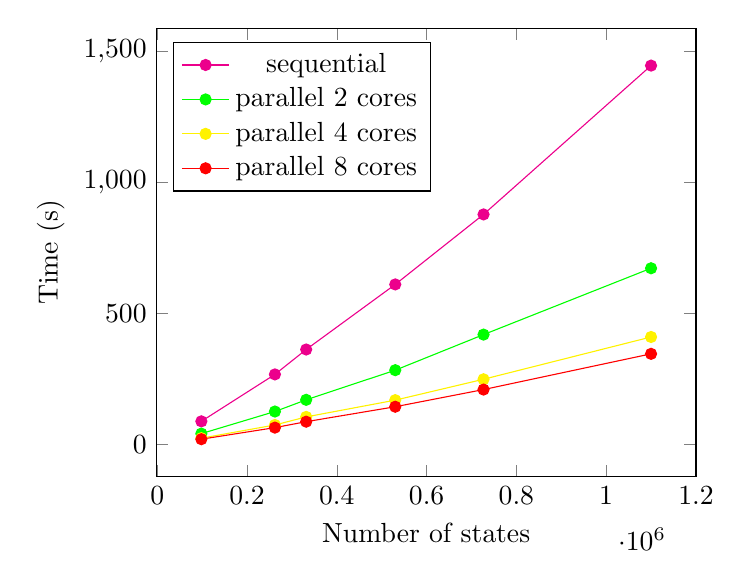
\begin{tikzpicture}
\definecolor{color0}{rgb}{0.75,0,0.75}

\begin{axis}[legend style={legend pos=north west},
ylabel={Time (s)},
xlabel={Number of states},
legend entries={{sequential},{parallel 2 cores},{parallel 4 cores},{parallel 8 cores}}
% scaled ticks=false
]

% Sequential
\addplot [magenta, mark=*, mark size=2pt]
coordinates {
(98279,     88.633369210) 
(262144,   267.658476596) 
(331776,   362.664597933) 
(530202,   610.926546563) 
(726836,   878.042343995) 
(1099999, 1445.821632163) 
};

% 2
\addplot [green, mark=*, mark size=2pt]
coordinates {
(98279,    41.786394435)
(262144,  126.064339906)
(331776,  170.664153825)
(530202,  283.808419361)
(726836,  419.506128369)
(1099999, 672.649284048)
};

% 4
\addplot [yellow, mark=*, mark size=2pt]
coordinates {
(98279,    24.373880968) 
(262144,   74.762257833) 
(331776,  105.559247500)
(530202,  169.459170682)
(726836,  249.133023117)
(1099999, 410.412285810)
};

% 8
\addplot [red, mark=*, mark size=2pt]
coordinates {
(98279,    20.521322935)  
(262144,   64.652309353)  
(331776,   87.323938113) 
(530202,  144.356493902) 
(726836,  209.819065630) 
(1099999, 346.097981548) 
};


\end{axis}
\end{tikzpicture}

}\hfill
\subcaptionbox{The relevant speedup gained over the sequential algorithm running our parallel algorithm with 100 states per thread and an increasing number of virtual cores. The graph shows that for each increase in the number of virtual cores we see a consistent speedup.} {
    \setfigname{}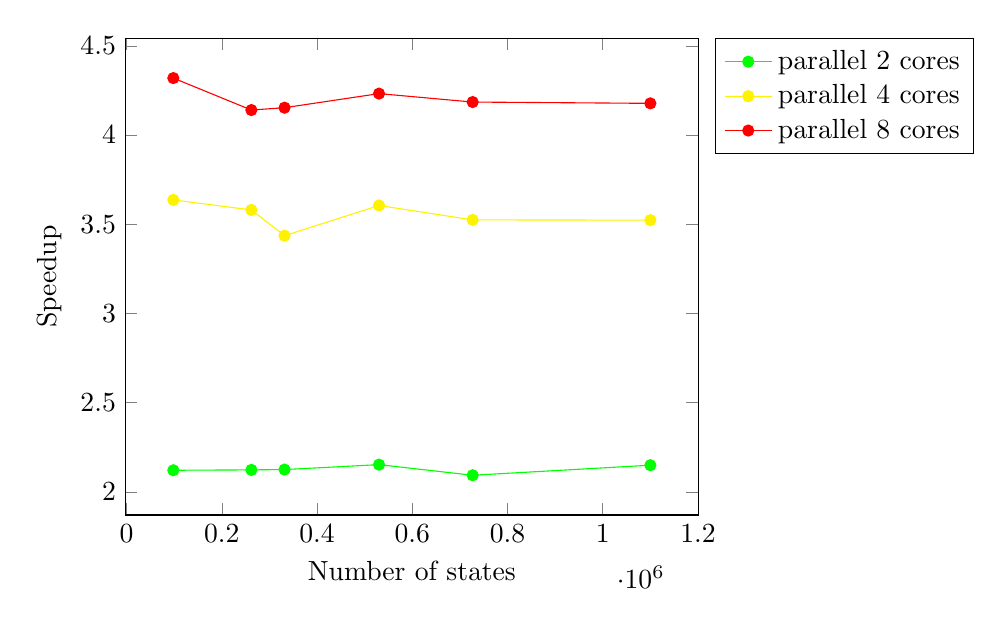
\begin{tikzpicture}
\definecolor{color0}{rgb}{0.75,0,0.75}

\begin{axis}[width=0.73\textwidth,
legend style={legend pos=outer north east},
ylabel={Speedup},
xlabel={Number of states},
legend entries={{parallel 2 cores},{parallel 4 cores},{parallel 8 cores}}
% scaled ticks=false
]

% 2
\addplot [green, mark=*, mark size=2pt]
coordinates {
(98279,   2.1211059343220406) % 99860326918 / 51611435904
(262144,  2.1231894506851012) % 304887660912 / 158793100442 
(331776,  2.1250191666193614) % 407267170985 / 208514610650
(530202,  2.152601913426362) % 709773626643 / 362338733157
(726836,  2.093038181369949) % 1023339231997 / 523542258224
(1099999, 2.149443501169068) % 1621045044327 / 845268409674
};

% 4
\addplot [yellow, mark=*, mark size=2pt]
coordinates {
(98279,   3.6364077319637786) % 99860326918 / 30575984607
(262144,  3.5801283208150485) % 304887660912 / 93863598681
(331776,  3.43564970878558) % 407267170985 / 127750195215
(530202,  3.605154823455611) % 709773626643 / 215606239138
(726836,  3.5243916402950974) % 1023339231997 / 318285464137
(1099999, 3.522851732641215) % 1621045044327 / 515475748470
};

% 8
\addplot [red, mark=*, mark size=2pt]
coordinates {
(98279,   4.319086517508672) % 99860326918 / 26825872545
(262144,  4.139967764099366) % 304887660912 / 82619391439
(331776,  4.153094853139814) % 407267170985 / 110556083237
(530202,  4.232068333397891) % 709773626643 / 189352805147
(726836,  4.184759575392262) % 1023339231997 / 282687963976
(1099999, 4.177492239903399) % 1621045044327 / 456685753436
};


\end{axis}
\end{tikzpicture}

}
\hspace*{\fill}%
\caption{A comparison between the run-times and relevant speedup of PIPE 5's sequential state space exploration and its parallel algorithm with 100 states per thread running on 2, 4 and 8 virtual cores on a 3.2GHz quad-core hyper-threaded 3rd generation i7 processor.}
\label{fig:scalability}
\end{figure}